\subsubsection{Merging of datasets by recalling prior to refinement and phasing}
Following curation of individual datasets, these will need to be merged to homogenise variant calls across all data, and generate a non-sparse matrix of variant calls, where the union of variants across all samples is available for each population. This process is similar to the merger of reference panels by imputation (Figure \ref{fig:merging_reference_panels}), which could have been used, if raw reads had not been available for all populations. In order to fill the sparse matrix a union set of calls will be generated for variants that have passed filtering in each dataset (Figure \ref{fig:calling}). Prior to merging we recode any haploid male genotypes (non-PAR X and Y) to homozygous diploid genotypes if necessary. %Prior to merging 1) indels will be left aligned (e.g. bcftools norm) and 2) SNPs and indels called in low coverage data by UnifiedGenotyper will be merged into single records with bcftools (bcftools norm -m +any).
%and 3) variants called from reads aligned to build 38 will be lifted over to build 37 (liftOver). %http://hgdownload.soe.ucsc.edu/admin/exe/linux.x86_64/liftOver
Variants will be merged across cohorts (with bcftools merge $|$ bcftools view -G instead of GATK CombineVariants \texttt{--}minimalVCF, because the latter creates multiple records at the same position, but UG in GGA mode only considers the first record).
%WARN  10:17:31,834 GenotypingGivenAllelesUtils - Multiple valid VCF records detected in the alleles input file at site 20:570945, only considering the first record 
These sites will then be recalled in each dataset to generate genotype likelihoods at these sites.
%Sample NA12878 will not be part of the recalling and NA12878 singletons will not be called by exclusion from the union set.
%Where necessary the union set of sites will be lifted over to build 38 prior to recalling and the recalled variants will then be lifted back over to build 37.
\gls{UG} will be used for recalling in GGA mode (\texttt{-{}-}genotyping\_mode GENOTYPE\_GIVEN\_ALLELES and \texttt{--}output\_mode EMIT\_ALL\_SITES).
%http://gatkforums.broadinstitute.org/discussion/4936/not-all-sites-emitted-with-genotype-given-alleles
The maximum number of allowed alternate alleles will be kept at the default 6, since indels are not being called. %Although it should only be necessary for HaplotypeCaller, interval padding will be added to ensure all known sites are called (--interval\_padding 100). %Not necessary for UG.
%http://gatkforums.broadinstitute.org/discussion/comment/18353
Following this, genotype refinement will be carried out, because we have shown refinement to improve genotype likelihoods for especially rare variants for low coverage data\cite{Gurdasani2015}.

\begin{figure}[htbp]
\centering
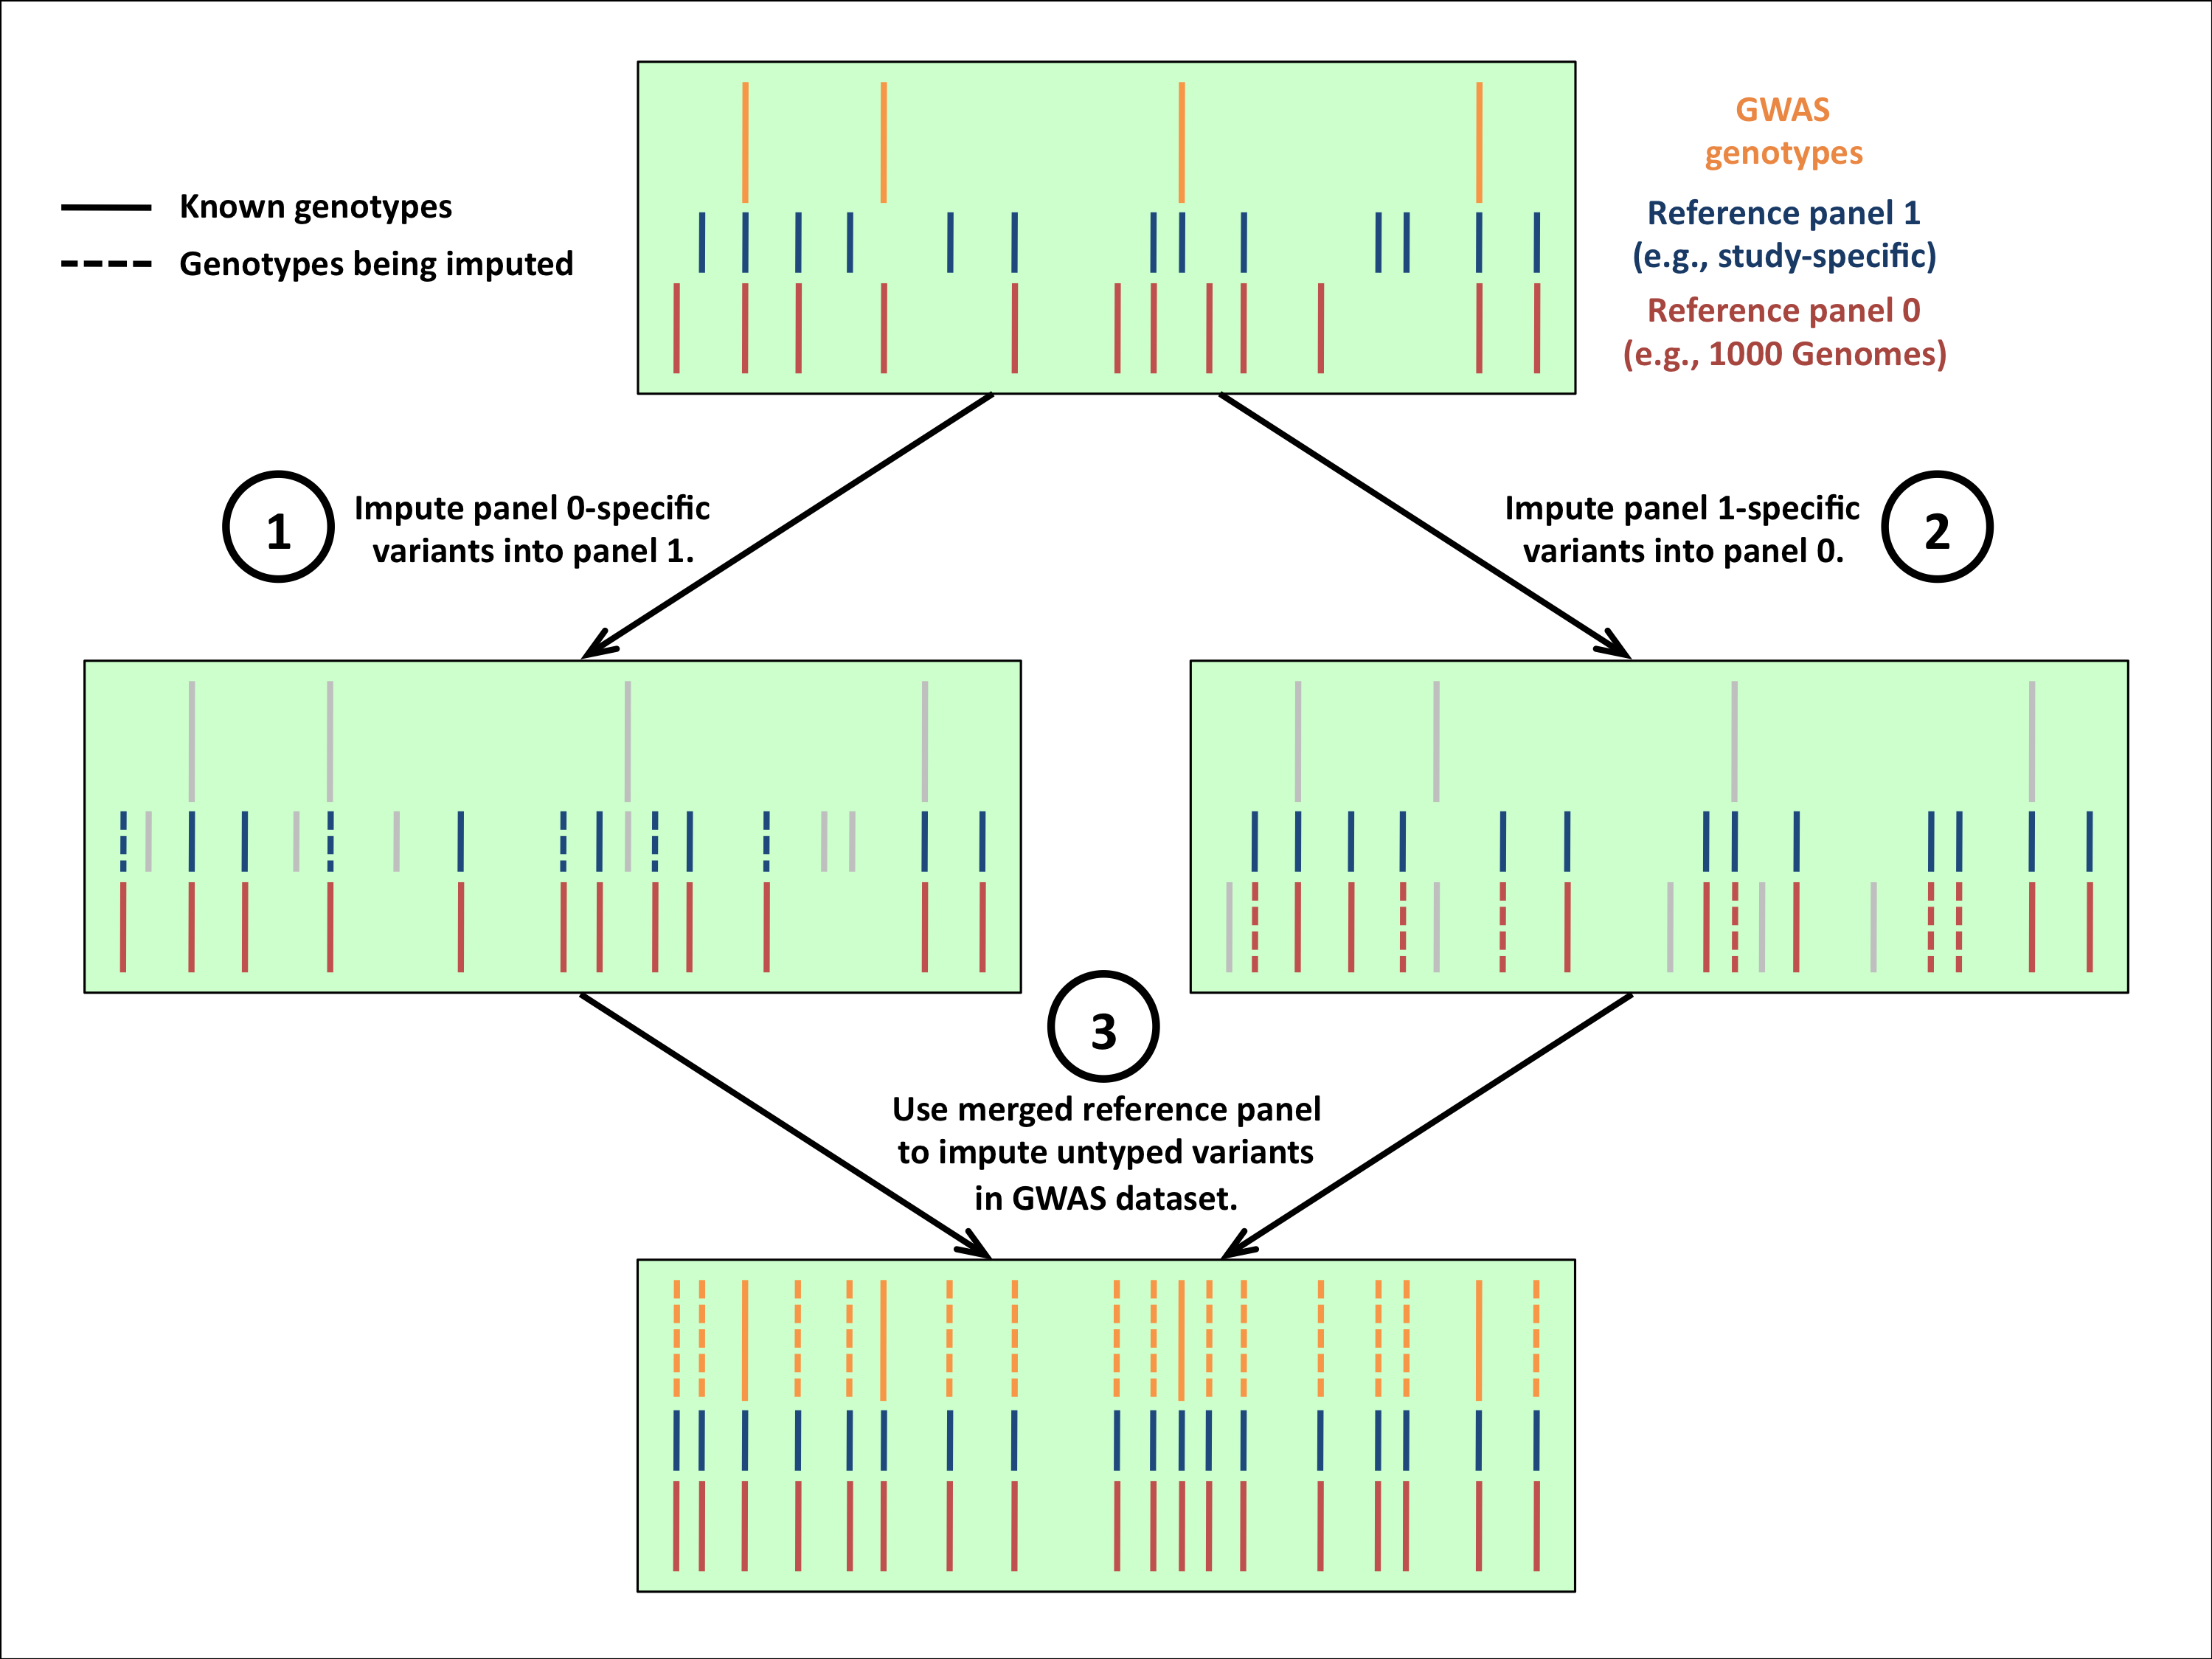
\includegraphics[width=0.6\textwidth]{merging_reference_panels}
\caption{The principle of creating a non-sparse matrix is the same as the merger of reference panels by imputation software. Figure copied from \href{http://mathgen.stats.ox.ac.uk/impute/merging\_reference\_panels.png}{IMPUTE2 web site}.}
\label{fig:merging_reference_panels}
\end{figure}

The detailed work flow is:
\begin{enumerate}
\item{Create \texttt{-{}-}alleles input files for the recalling with \gls{GATK} \gls{UG} run with \texttt{-{}-}genotyping\_mode GENOTYPE\_GIVEN\_ALLELES.}

\begin{enumerate}

\item{Split multiallelic variants into biallelic variants using bcftools norm (-m -) and left align indels (-f) to enable comparison of individual alternate alleles at multiallelic sites by bcftools isec.}

\item{Filter out complex variants from the dataset and 1000Gp3 calls using bcftools view (-v snps).}

\item{Find the union set of sites in the ADRP and 1000Gp3 calls using bcftools isec (-n+1).}

\item{Merge multiallelic sites into one VCF record with bcftools norm (-m +any) to avoid GATK UG only considering the first record.}

\end{enumerate}

\item{Run \gls{GATK} \gls{UG} with \texttt{--}genotyping\_mode GENOTYPE\_GIVEN\_ALLELES across all samples of both datasets.}

%2nd VR because either false sites, false genotypes or UG fail.
\item{Because we found the 1000G samples to cluster together in a PCA plot \ref{fig:PCAprepostVR} we ran another round of \gls{VR} after the joint calling of the union set. We applied a truth sensitivity threshold of 99.5\% after plotting the sensitivity and false discovery rate as a function of VQSLOD scores
%(figure \ref{ROC2}).
. Prior to the second round of \gls{VR} we also exclude variants with a non-reference allele count of 0 (table \ref{tab:SNPcount}), which could be due to a different genotype being called for rare variants during the joint calling of the union set or the variant being called in 1000G by a method involving local realignment, which is not part of \gls{GATK} \gls{UG}. Many of these variants are singletons, which were also excluded as part of the UK10K efforts to generate a merged reference panel.\cite{2015Huang}}

\item{Exclusion of samples in each population with a heterozygosity deviating more than 3.5 standard deviations from the mean for each population (table \ref{tab:samplecount}).}

\item{Refinement with Beagle4 and phasing with SHAPEIT2 as described in section \ref{sec:refine_and_phase}.}

\end{enumerate}

\begin{figure}[h]
\begin{subfigure}{.5\textwidth}
  \centering
  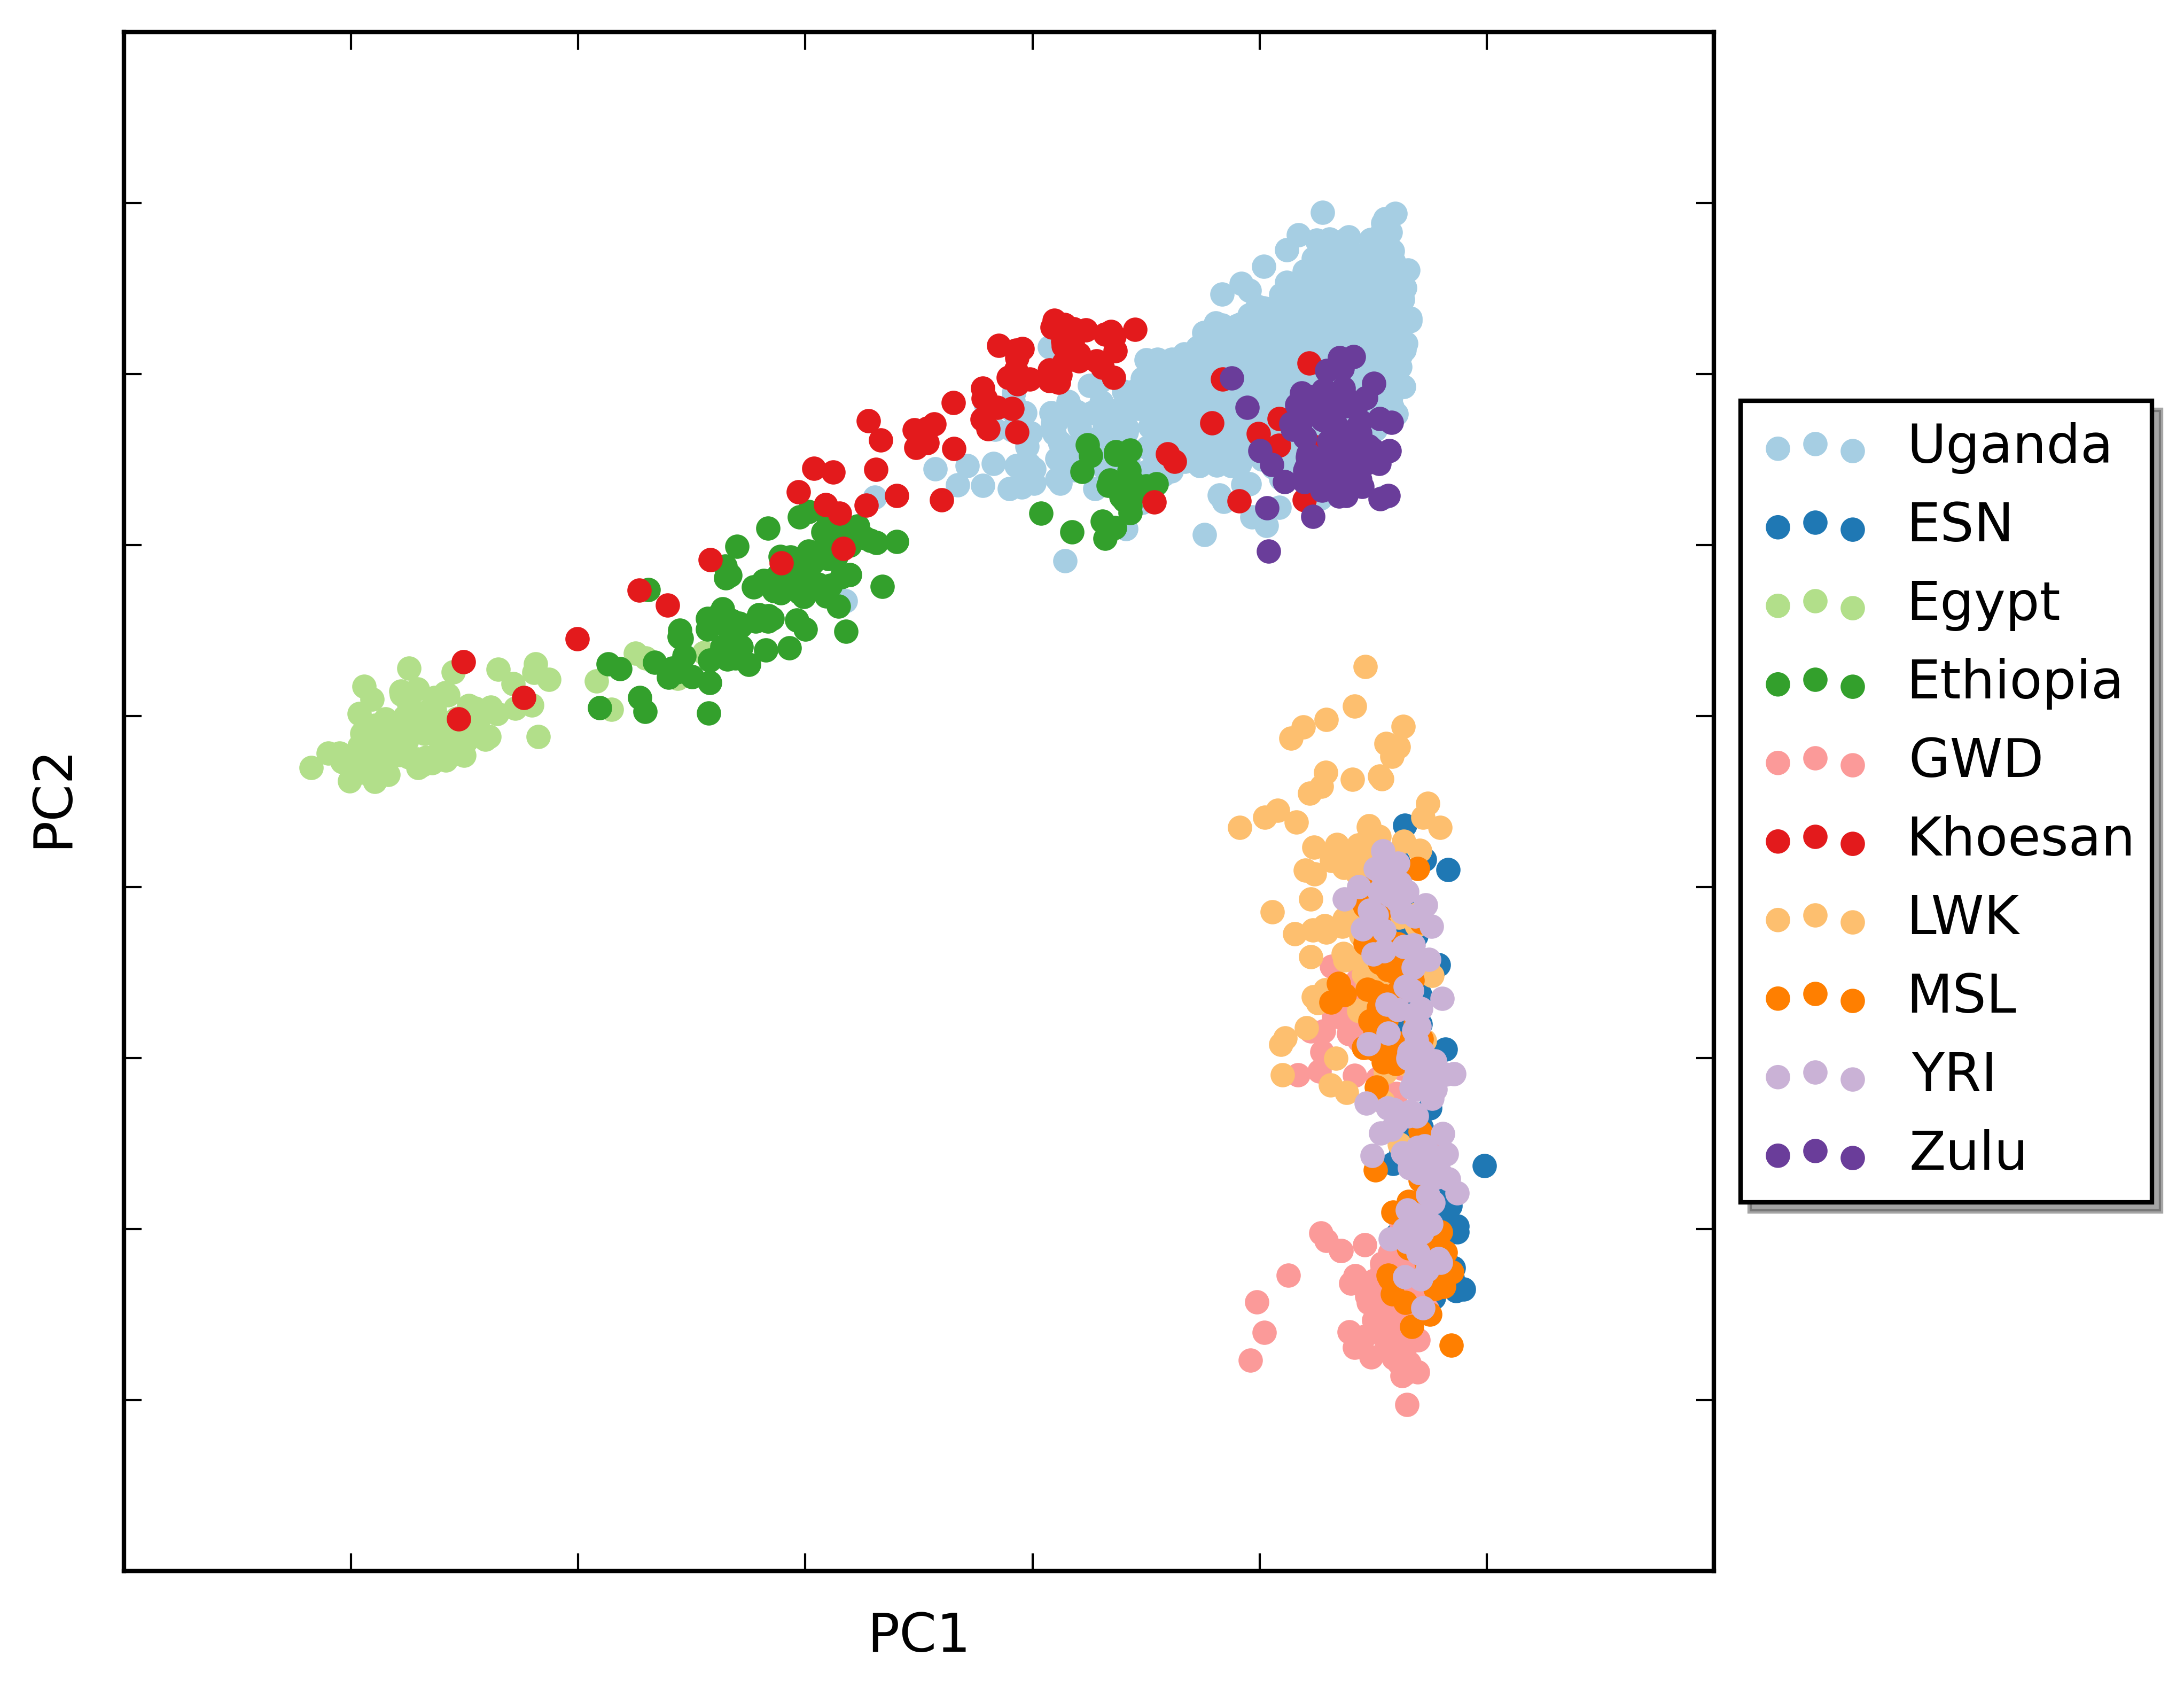
\includegraphics[width=1.0\linewidth]{ADRP/figures/PC12_africa_noVR.png}
  \caption{}
\end{subfigure}%
\begin{subfigure}{.5\textwidth}
  \centering
  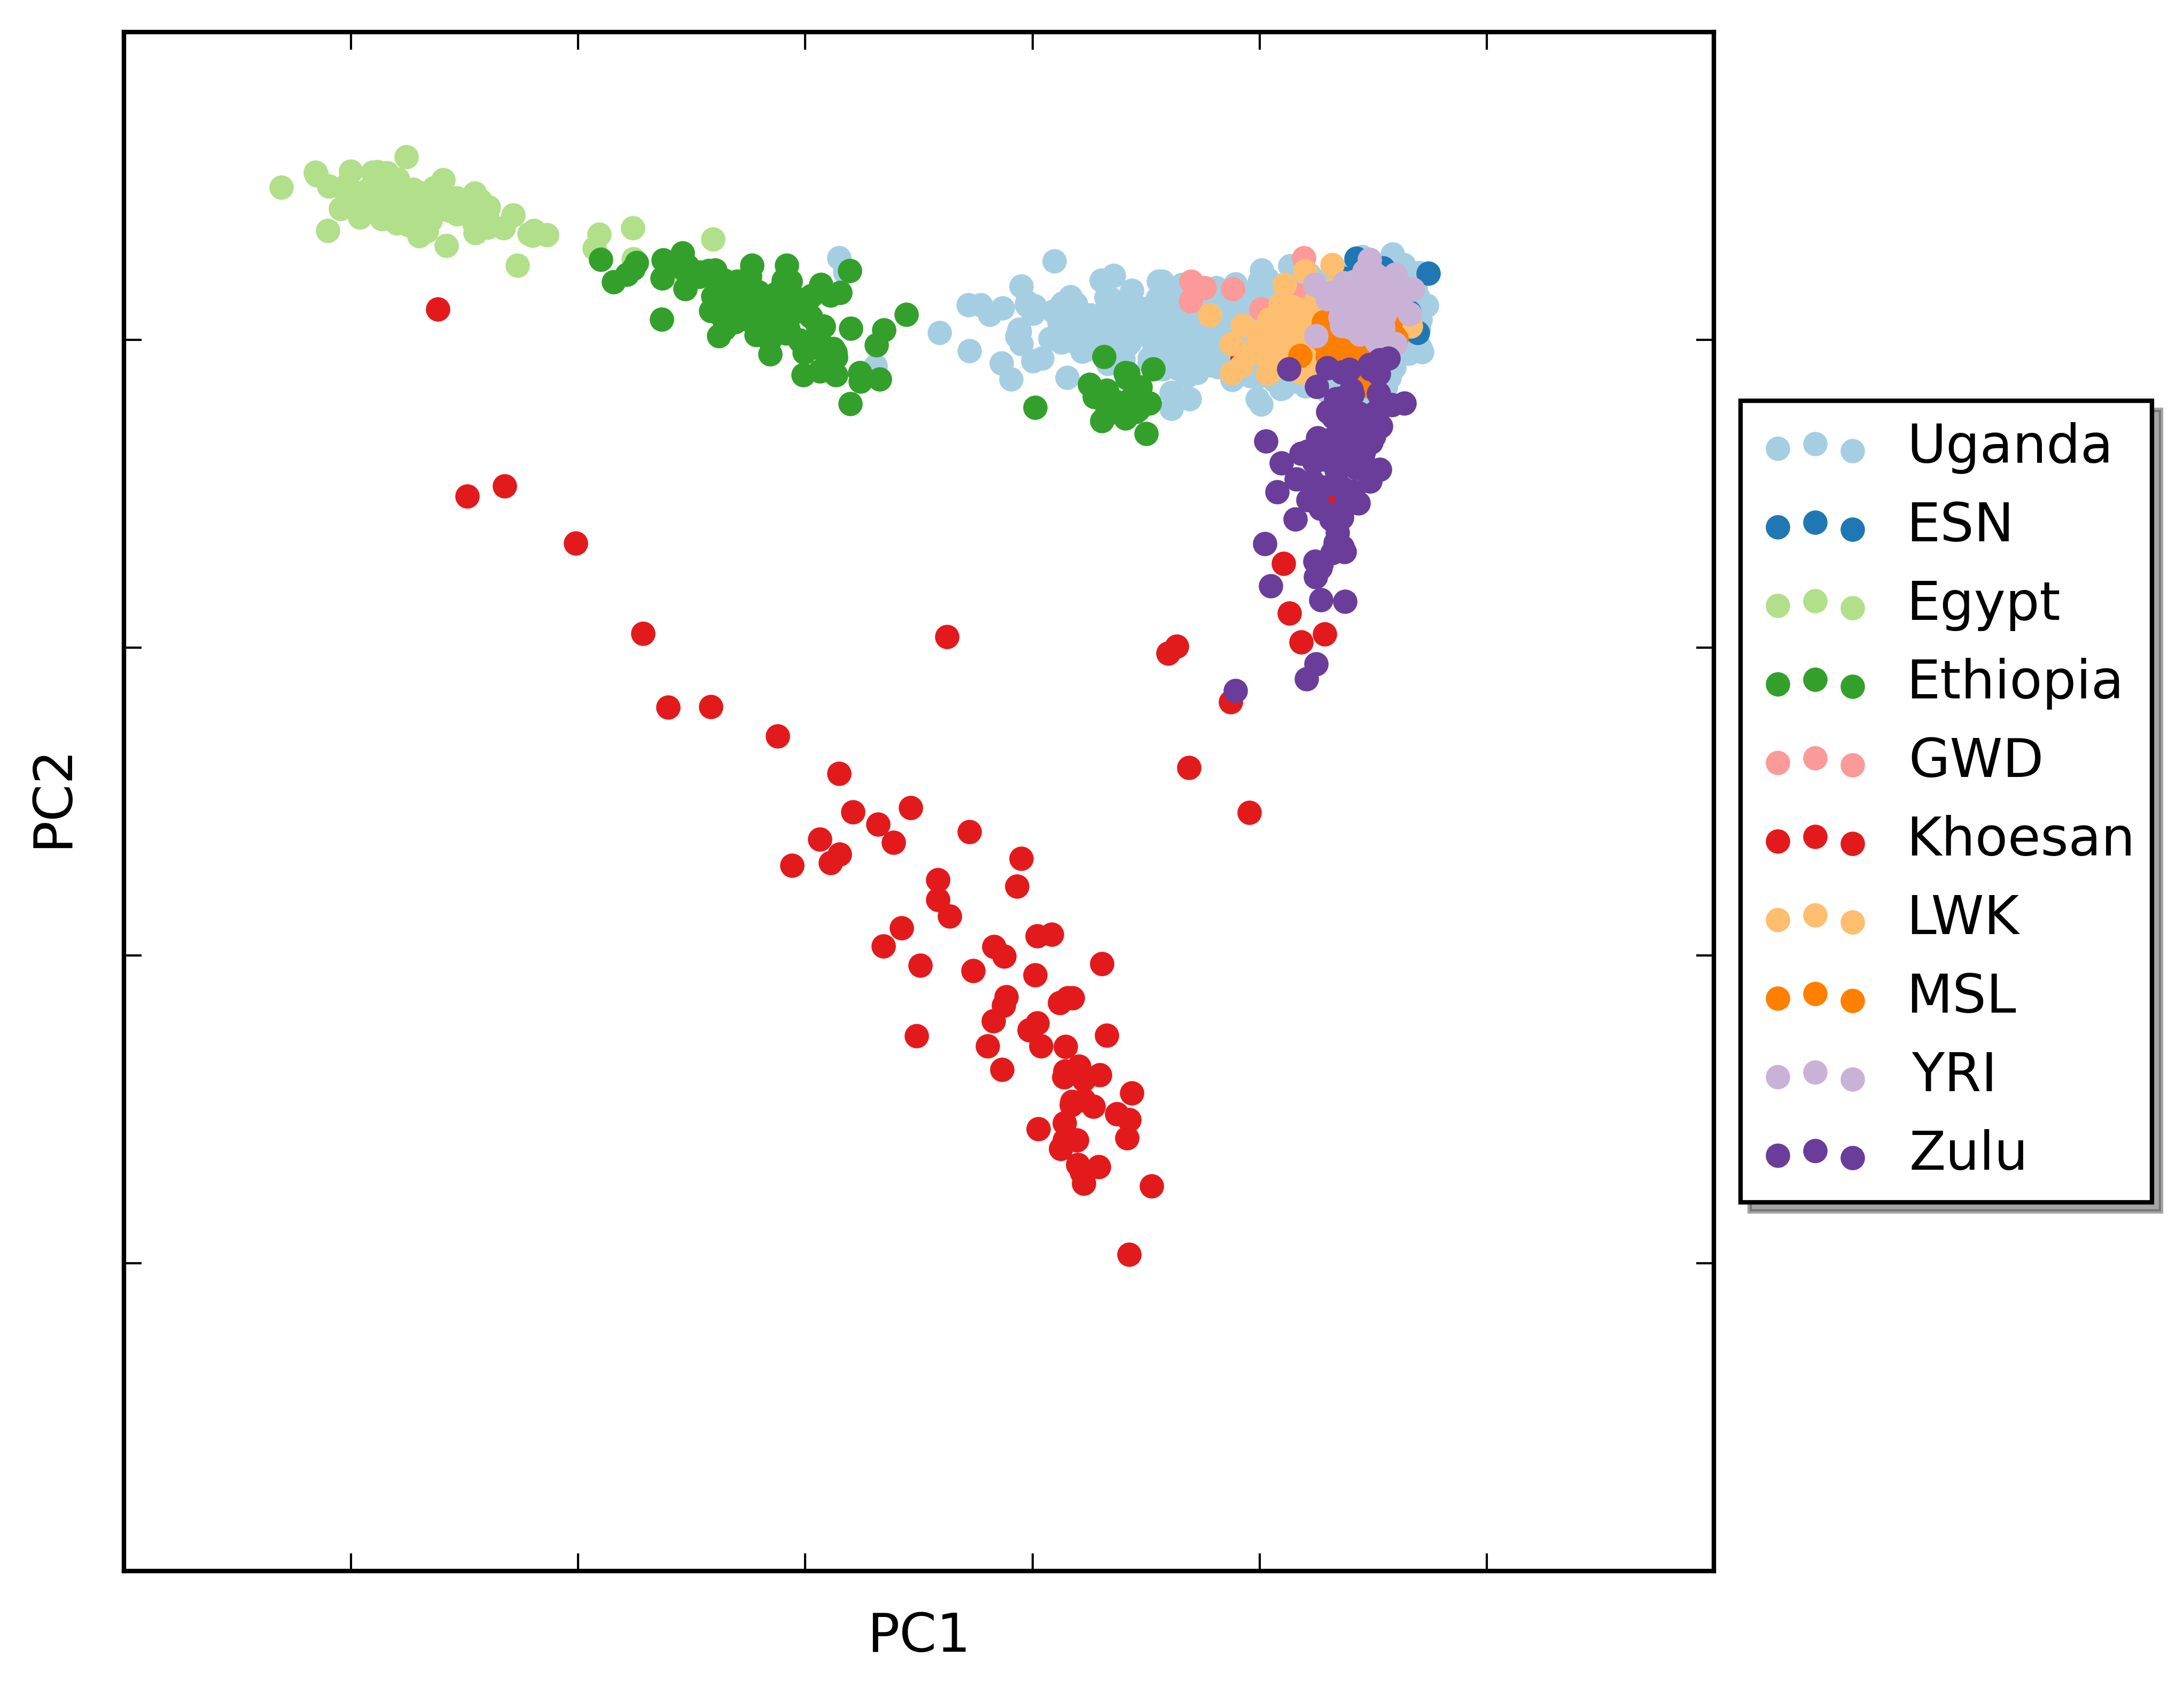
\includegraphics[width=1.0\linewidth]{ADRP/figures/PC12_africa}
  \caption{}
\end{subfigure}%
\caption{Plots of principal components 1 and 2 for 3055 African samples prior to refinement without (a) and with (b) a 2nd round of \gls{VR}. The LWK samples from East Africa can be seen to cluster with the 4 1000G populations from West Africa, if a 2nd round of \gls{VR} is not carried out, which filters out approximately 10 million variants.}
\label{fig:PCAprepostVR}
\end{figure}

The sample count after each step of the curation process is summarised in table \ref{tab:samplecount}.

The SNP count after merger with 1000G and re-calling of the union set of sites jointly across all samples is summarised in table \ref{tab:SNPcount}.

Prior to refinement we check the correlation with chip data (table \ref{tab:correlation_prerefinement} and figure \ref{fig:correlation_prerefinement})

\begin{table}[htbp]
\centering
\begin{tabular}{l|r|r|r|r}
\hline
Population & Sample Intersection Count & Median & Min & Max \\
\hline
Baganda & 435 & 0.806 & 0.544 & 0.946 \\
Zulu & 67 & 0.824 & 0.674 & 0.934 \\
Ethiopia & 61 & 0.922 & 0.760 & 0.957 \\
Khoesan & 79 & 0.885 & 0.544 & 0.965 \\
Egypt & 97 & 0.943 & 0.770 & 0.979 \\
\hline
\end{tabular}
\caption[Correlation between sequence calls and SNP array genotypes prior to refinement.]{Correlation between sequence calls and chip calls for each population on chromosome 20 prior to refinement after exclusion of heterozygosity outliers.}
\label{tab:correlation_prerefinement}
\end{table}

\begin{figure}[h]
    \centering
    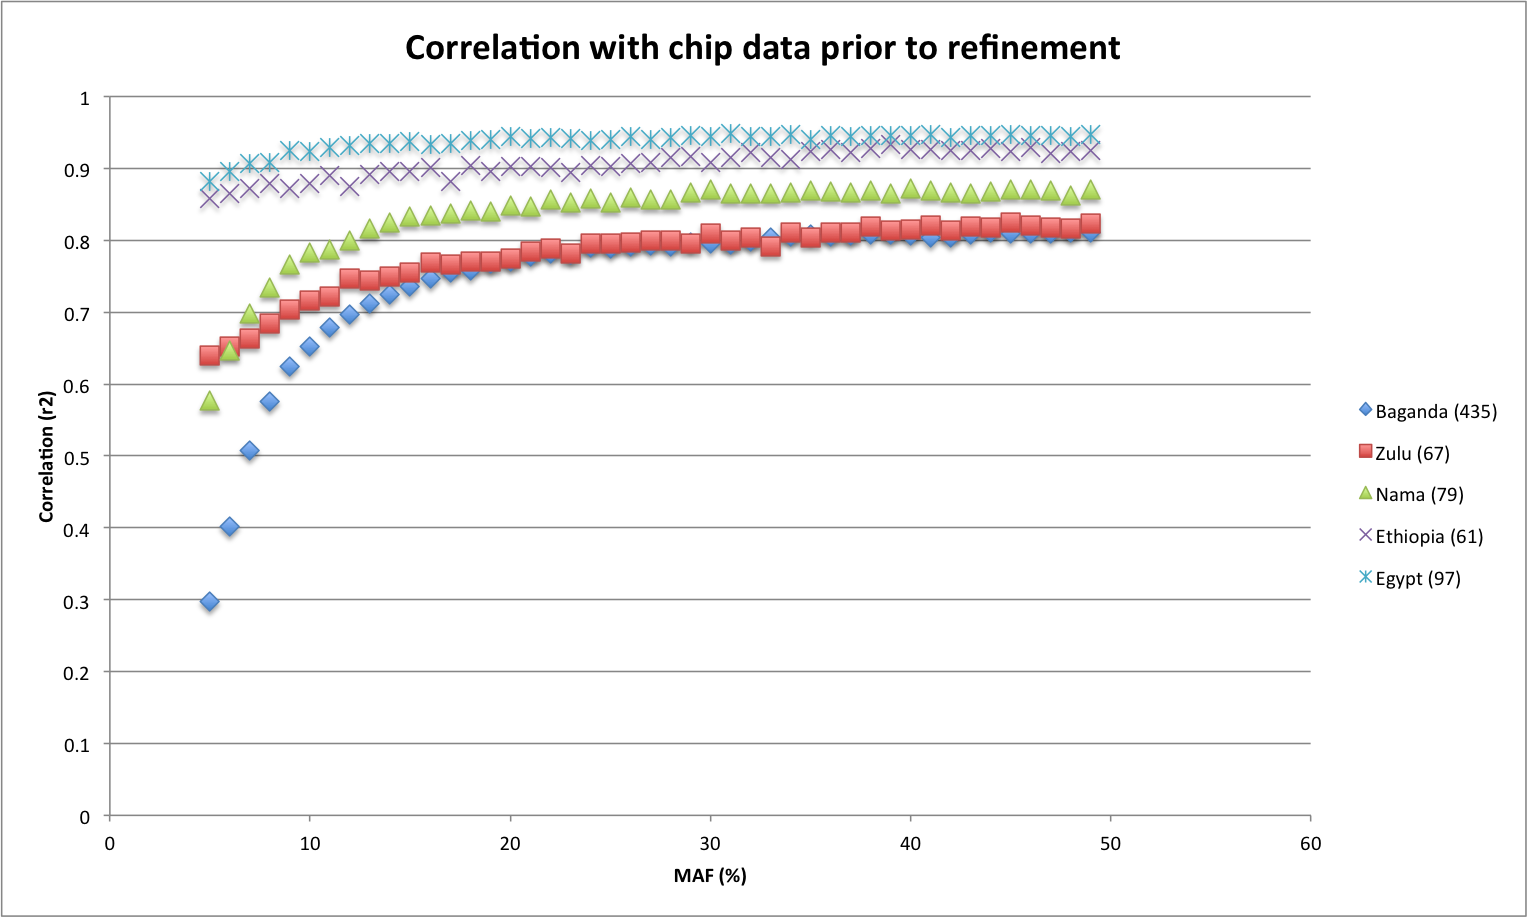
\includegraphics[width=0.8\textwidth]{correlation_prerefinement}
    \caption{Correlation between Omni2.5 chip data and SNP calls prior to refinement.}
    \label{fig:correlation_prerefinement}
\end{figure}

\begin{table}[htbp]
\centering
\begin{tabular}{l|r|r|r|r}
 & Sequencing & QC & verifyBamID & Heterozygosity \\
\hline
Baganda & 1667 & 1656 & 1647 & 1637 \\
Banyarwanda & 199 & 198 & 197 & 196 \\
Barundi & 51 & 51 & 51 & 51 \\
Banyankole & 36 & 36 & 36 & 36 \\
Bakiga & 30 & 30 & 30 & 30 \\
Rwandese Ugandan & 76 & 74 & 74 & 74 \\
Uganda, Other & 41 & 41 & 41 & 41 \\
Zulu & 100 & 98 & 98 & 98 \\
Wolayta & 24 & 24 & 24 & 24 \\
Somali & 24 & 24 & 24 & 24 \\
Oromo & 24 & 24 & 24 & 24 \\
Gumuz & 24 & 23 & 23 & 23 \\
Amhara & 24 & 22 & 22 & 22 \\
Egypt & 100 & 100 & 100 & 100 \\
Khoesan & 111 & 107 & 86 & 85 \\
LWK & 99 & N/A & N/A & 99 \\
GWD & 113 & N/A & N/A & 113 \\
MSL & 85 & N/A & N/A & 85 \\
ESN & 99 & N/A & N/A & 99 \\
YRI & 108 & N/A & N/A & 108 \\
1000Gp3 (nonAFR, ASW, ACB) & 2000 & N/A & N/A & 2000 \\
\hline
 &  &  &  &  \\
Sum & 5035 & 5012 & 4981 & 4969
\end{tabular}
\caption[Count of samples after each step of the curation process.]{Count of samples after each step of the curation process. N/A means that curation step was not carried out for that data set. Sequencing is the number of sequenced samples. QC is the initial QC process adapted from UK10K. verifyBamID is the subsequent check for contaminated samples with excess heterozygosity and swapped samples. Heterozygosity is the check of heterozygosity outliers after recalling variants prior to refinement with Beagle4.}
\label{tab:samplecount}
\end{table}

\begin{table}[htbp]
\centering
\resizebox{\textwidth}{!}{%
\begin{tabular}{l|r|r|r|r|r|r|r}
\hline
Chromosome & UG1 & VR1 & 1000G & Union & UG2 & non-monomorphic & VR2 \\
\hline
1 & 7331048 & 4466570 & 6238533 & 8135665 & 8135665 & 8121685 & 7220178 \\
2 & 7563940 & 4897414 & 6834236 & 8930898 & 8930898 & 8916004 & 8057100 \\
3 & 6126618 & 4062320 & 5624615 & 7347008 & 7347008 & 7335431 & 6679331 \\
4 & 5935191 & 3981077 & 5521818 & 7161759 & 7161759 & 7149973 & 6461409 \\
5 & 5556780 & 3690538 & 5075395 & 6650082 & 6650082 & 6639451 & 6028368 \\
6 & 5373212 & 3516545 & 4835905 & 6282890 & 6282890 & 6272096 & 5660253 \\
7 & 5309419 & 3316764 & 4550705 & 5945705 & 5945705 & 5935472 & 5260940 \\
8 & 4813382 & 3232251 & 4453379 & 5821226 & 5821226 & 5812359 & 5290591 \\
9 & 3974961 & 2468538 & 3441213 & 4495196 & 4495196 & 4487714 & 3979574 \\
10 & 4434086 & 2804022 & 3852282 & 5018268 & 5018268 & 5009565 & 4493579 \\
11 & 4287471 & 2802106 & 3907160 & 5084045 & 5084045 & 5075931 & 4571193 \\
12 & 4347647 & 2710326 & 3724286 & 4863404 & 4863404 & 4854889 & 4363342 \\
13 & 2979117 & 2006917 & 2747376 & 3578012 & 3578012 & 3571947 & 3268732 \\
14 & 2933699 & 1855954 & 2558184 & 3334587 & 3334587 & 3328925 & 2994394 \\
15 & 2784077 & 1680149 & 2337651 & 3049792 & 3049792 & 3044491 & 2693114 \\
16 & 3169848 & 1856110 & 2619149 & 3422074 & 3422074 & 3416016 & 2976742 \\
17 & 3000276 & 1631664 & 2243354 & 2945166 & 2945166 & 2939413 & 2540165 \\
18 & 2390213 & 1595328 & 2187123 & 2848151 & 2848151 & 2843612 & 2587971 \\
19 & 2636969 & 1319309 & 1765908 & 2328868 & 2328868 & 2323718 & 1936939 \\
20 & 2091941 & 1288813 & 1751797 & 2294718 & 2294718 & 2290949 & 2076370 \\
21 & 1307809 & 770704 & 1063228 & 1376114 & 1376114 & 1373478 & 1205255 \\
22 & 1427343 & 782316 & 1064502 & 1396629 & 1396629 & 1393869 & 1192106 \\
X & 3838312 & 2280287 & 3261471 & 4260245 &  &  &  \\
 &  &  &  &  &  &  &  \\
\hline
Sum & 93,613,359 & 59,016,022 & 81,659,270 & 106,570,502 & 102,310,257 & 102,136,988 & 91,537,646 \\
\end{tabular}
}
\caption[\gls{SNP} count after each \gls{ADRP} data curation step.]{Count of SNPs after each step of the curation process. UG1 is an abbreviation for UnifiedGenotyper calls from the ADRP populations. VR1 is an abbreviation for variants passing the first VariantRecalibrator filtering. 1000G is a count of variants in 1000G. Union is a count of variants in the union set, which are recalled with UG. non-monomorphic is a count of the non-monomorphic SNPs after re-calling. VR2 is an abbreviation for passing the second round of VariantRecalibrator filtering.}
\label{tab:SNPcount}
\end{table}